%-----------------------------------------------------------------------------
%
%               Template for sigplanconf LaTeX Class
%
% Name:         sigplanconf-template.tex
%
% Purpose:      A template for sigplanconf.cls, which is a LaTeX 2e class
%               file for SIGPLAN conference proceedings.
%
% Guide:        Refer to "Author's Guide to the ACM SIGPLAN Class,"
%               sigplanconf-guide.pdf
%
% Author:       Paul C. Anagnostopoulos
%               Windfall Software
%               978 371-2316
%               paul@windfall.com
%
% Created:      15 February 2005
%
%-----------------------------------------------------------------------------


\documentclass[preprint]{sigplanconf}

% The following \documentclass options may be useful:

% preprint      Remove this option only once the paper is in final form.
% 10pt          To set in 10-point type instead of 9-point.
% 11pt          To set in 11-point type instead of 9-point.
% numbers       To obtain numeric citation style instead of author/year.

\usepackage{amsmath}
\usepackage{graphicx}
\usepackage{amsthm}
\usepackage{listings}

\newcommand{\cL}{{\cal L}}

\newcommand{\func}[1]{{\sc #1}}
\newcommand{\tabulate}{\func{tabulate}}
\newcommand{\get}{\func{get}}
\newcommand{\set}{\func{set}}
\newcommand{\tget}{\text{\get}}
\newcommand{\tset}{\text{\set}}
\newcommand{\ttab}{\text{\tabulate}}

\begin{document}

\special{papersize=8.5in,11in}
\setlength{\pdfpageheight}{\paperheight}
\setlength{\pdfpagewidth}{\paperwidth}

\conferenceinfo{CONF 'yy}{Month d--d, 20yy, City, ST, Country}
\copyrightyear{20yy}
\copyrightdata{978-1-nnnn-nnnn-n/yy/mm}
\copyrightdoi{nnnnnnn.nnnnnnn}

% Uncomment the publication rights you want to use.
%\publicationrights{transferred}
%\publicationrights{licensed}     % this is the default
%\publicationrights{author-pays}

% \titlebanner{banner above paper title}        % These are ignored unless
% \preprintfooter{short description of paper}   % 'preprint' option specified.

\title{A New Approach for Parallel Functional Arrays}

\authorinfo{Ananya Kumar}
           {Carnegie Mellon University}
           {ananyak@andrew.cmu.edu}
\authorinfo{Guy Blelloch}
           {Carnegie Mellon University}
           {blelloch@cs.cmu.edu}
\authorinfo{Robert Harper}
           {Carnegie Mellon University}
           {rwh@cs.cmu.edu}
\maketitle

\newtheorem{theorem}{Theorem}[section]
\newtheorem{corollary}{Corollary}[theorem]
\newtheorem{lemma}[theorem]{Lemma}
\theoremstyle{definition}
\newtheorem{definition}{Definition}[section]

\begin{abstract}
In this paper we introduce a $O(1)$ wait-free, parallel, functional array, that allows $O(1)$ reads and writes to the most recent version of the array. We describe the cost dynamics and sketch out a provable implementation. We show favorable benchmarks comparing our functional arrays with regular arrays in Java.
\end{abstract}

\category{CR-number}{subcategory}{third-level}

\keywords
array, parallel, cost semantics

\section{Introduction}
\label{sec:intro}

Supporting sequences (arrays) with efficient (constant time) random
access updates has been a persistent problem in functional languages
(pun intended).  It is easy to implement such sequences with constant
time random access reads (using arrays stored as contiguous memory),
or to implement with logarithmic time reads and updates using balanced
trees, but getting both in constant time cannot be done without some
form of extension.
%~\cite{Pippenger97}.  
This means that algorithms
for many fundamental problems are a logarithmic factor slower in
functional languages than in imperative languages.  This includes
algorithms for basic problems such as generating a random permutation,
and for many important graph problems (e.g.,
shortest-unweighted-paths, connected components, biconnected
components, topological sort, and cycle detection).  Simple algorithms
for these problems take linear time in the imperative setting, but an
additional logarithmic factor in time in the functional setting, at
least without extensions.

A variety of approaches have been suggested to alleviate this problem.
Many of the approaches are based on the observation that if there is
only a single reference to an array, it can be safely updated in
place.  The most common such approach is to use
monads~\cite{Moggi89,Wadler95}.  Monads can force code to be single
threaded and can thread mutable arrays (or other mutable
state) implicitly so the only reference to them is the current one.
Haskell supplies the ST monad for this purpose.  King and Launchbery,
for example, use STMonads with an array to implement depth first (DFS)
search in linear work~\cite{KL95}.  Guzman and Hudak's single-threaded
lambda calculus also uses the idea of single threading the
computation~\cite{GH90}, and motivate the approach based on allowing
for fast array updates.  The problem with using these approaches is
that it is basically implementing a second imperative language within
a functional language.  Using monads means using a new syntax not just
for the operations themselves but for everything the operations are
embedded in.  Indeed King and Launchbery have to write completely
different code for DFS, even though it is only for efficiency and not
correctness (it is trivial to implement DFS in $O(m \log n)$ time
purely functionally).  Monads also do not allow keeping persistent
versions of structures, exactly because the state can be changed.
More importantly, however, it forces the program itself to be single
threaded, inhibiting parallelism.

A second approach is to use a type system that enforces the
single-threadedness of individual arrays rather than the program as a
whole.  This can be done with linear types~\cite{Girard87,Wadler90},
which can be used to ensure that references are not duplicated.  This
is more flexible than monads, since it allows the threading of the
data to be distinct from the threading of the program.  However, such
type systems are not available in most languages, and they can be hard
to reason about.

A third approach is to support fully functional arrays in a general
functional language, and to check in the program if they happen to be
used in a single threaded manner.  This can be done, for example, by
using reference counting~\cite{HB85,Hudak86}.  The idea is to keep
track of how many references there are to an array and update inplace
if there is only one.  Hudak describes techniques to statically
analyze code to determine that at certain points in the code a count
must be one, and therefore it is safe to replace an update with an
inplace update.  The problem with this approach is that the efficiency
of the code depends heavily on the effectiveness of the compiler and
the specific way the code is written, and it can therefore be hard for
the user to reason about efficiency.

The last approach is to fully support functional arrays, even with
sharing, but more efficiently than as a simple array or tree.  This is
sometimes referred to as version tree arrays~\cite{AHN88} or fully
persistent arrays~\cite{DSST89}.  The idea is to maintain a version
tree for an array (or more generally other data types), such that any
node of the tree can be updated to create a new leaf below it with the
modified value, without effecting the value of other nodes.  Dietz
showed that arrays can be maintained fully persistently using
$O(\log\log n)$ time per operation (read or write).  Holmstrom, Hughes
and others (see \cite{AHN88}) suggested storing a version tree by
keeping the full array at the root, and a each node represents an
update.  Chuang's approach ~\cite{chuang} supports $O(1)$ accesses and
insertions to the most recent version of arrays, however accessing old
versions of the array takes $O(n)$ work which is often impractical.
O'Neill and Warren~\cite{oneill} describe various improvements.
The problem with these approaches is that they can be very complicated,
and only efficient in certain cases.   Furthermore it can be hard to
reason about the performance.

None of the existing approaches support concurrent operations on
arrays.  O' Neill suggests (in passing) having a lock for each element
of the array. However, when many threads contend for the same element,
this would serialize accesses and make accesses not
$O(1)$. Additionally, per-element locks add significant memory
overhead.  
% Separation logic ~\cite{reynolds} could be used to
% parallelize divide and conquer algorithms on arrays however they would
% severely restrict the way functional arrays can be used.

\subsection*{Our Approach}

In this paper we present an approach for efficiently supporting
functional arrays.  It uses some ideas from the previous approaches
but unlike the previous approaches it supplies a well
defined cost semantics, and supports parallelism, and without language
extensions.  More specifically the approach has the
following important features.
\begin{enumerate}
\item It has fully functional value semantics (dynamic
  semantics)---i.e., when not considering costs, arrays act no
  differently than purely functional arrays.
\item It requires no changes in existing languages and no special
  types, syntactic extensions, etc.  Programs can be efficient---i.e.,
  constant time reads and writes---when using a completely standard
  functional programming style.
\item The approach supports nested parallelism---arrays can be passed
  to parallel calls and safely updated and read, again with a purely
  functional semantics.
\item We supply a well defined cost semantics, which can be used to
  formally analyze the cost of any program.  The semantics captures
  both sequential and parallel costs.
\item We describe a cost-bounded implementation which maps costs in the
  model to costs on either a sequential or parallel RAM (PRAM).
\item
Although accessing old versions of an array is more expensive than
accessing new versions (as defined in the cost semantics), reading old
versions never costs more than $O(\log n)$ work.
\end{enumerate}
We have implemented the approach and in this paper present some
performance numbers.

Although our value semantics are purely functional (and compositional)
our cost semantics are not---they require passing a store and modeling
costs based on the order the store is threaded.  The reader might
object to this non-functional nature of the cost semantics, but we
note that non-functional costs are also requires in call-by-need
(lazy) languages, which supply a functional value semantics but an
imperative cost semantics.  In fact from the value point of view,
call-by-need is no different from call-by-name, and it is only when
considering costs that they differ.  The cost semantics of
call-by-need~\cite{AMOFW95} is completely non-functional
(non-compositional).  Furthermore it is likely significantly more
complicated to reason about than the cost semantics we present in this
paper.

\begin{figure}[!ht]
\centering 
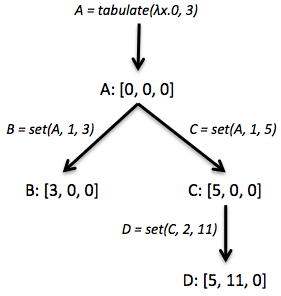
\includegraphics[scale=0.45]{leaf_interior_intro}
\nocaptionrule \caption{Example usage of functional arrays}
\label{fig:leaf_interior_intro}
\end{figure}

In this paper we consider arrays with three functions: \tabulate{},
\get{} (read), and \set{} (write).  As usual, \tabulate{}$(f,n)$
creates a new array of length $n$ by applying the function $f$ to
$[0, \ldots, n-1]$, \get$(A,i)$ returns the $i^{th}$ element of $A$, and
\set$(A,i,v)$ sets the $i^{th}$ element of $A$ to $v$ returning a
``new'' array (in the following discussion $n$ refers to the length of
an array).  Figure~\ref{fig:leaf_interior_intro} gives an example.  As
in previous work~\cite{AHN88} the history of an array after it is
created with \tabulate{} can be viewed as a version tree.  A version
tree has interior nodes and leaves.  In the figure, after all
functions are applied, arrays $A$ and $C$ are \emph{interior nodes},
and arrays $B$ and $D$ are \emph{leaves} of the version tree.  In our
cost semantics applying \get{} and \set{} to arrays at the leafs takes
constant work, but applying them to interior nodes is more expensive.
We define a cost semantics that identifies whether an array is a leaf
or interior node and charges for the cost of \get{} and \set{}
appropriately.  This requires threading a store that maps labels
(corresponding to each array) to indicate whether the array is a leaf
or interior.

Since we are also interested in parallelism, we include fork-join
parallelism in our language and semantics.    Our cost semantics then
models the cost of arrays when used in parallel.  This is non-trivial
since parallel tasks can read and update an array in parallel.
To deal with this, we compute the work of each forked task separately,
and then charge additional work at the join point if an array is used
in both forks.

To implement our functional arrays, we maintain at each leaf of the
version tree an array of the most recent values.  We also keep with
each location a change-log that keeps track of values at interior
nodes of the version tree.  Applying \get{} to a leaf only requires a
lookup in the array.  Applying \set{} to a leaf only requires updating
the array, and adding an element to the change log for the old
version.  Applying \get{} to an interior nodes requires a binary
search on the change log, which can be bounded by $O(\log n)$ time.
To ensure that change logs do not get too large, whenever the total
size across all change logs reaches $n$, the array is copied.   This
requires $O(n)$ time, but can be amortized against the updates.
Applying \set{} to an interior node requires creating a new array,
and copying values to it.   This requires $O(n)$ time.    

We give a wait-free concurrent implementation that uses careful
synchronization. We prove linearizability of the implementation and
use that to prove that our arrays work correctly when used
concurrently. Finally, we give a provable implementation for our cost
dynamics.



\section{Dynamics}

We use a standard applicative-order source language defined as follows:
$$e = x \; | \; c  \; | \; \lambda x.e \; 
| \; e_1 e_2 \; 
| \; (e_1, e_2) \; 
| \; (e_1 || e_2) \; 
| \; \text{if } e_1 \text{ then } e_2 \text{ else } e_3$$

The constants $c$ contains the usual arithmetic types, such as the
natural numbers and numerical functions.  The expression $(e_1||e_2)$
indicates that the two expressions can run in parallel, returning a
pair when both expressions are fully evaluated, and $(e_1,e_2)$
generates a pair sequentially.  The terminal (fully evaluated) values
are lambda expressions, as well as pairs and arrays of terminal
values, and are denoted by the judgement val.   Our value semantics are given by the judgement:
\[e \Downarrow v\]
indicating that the expression $e$ evaluates to $v$.  The rules for
function application and parallel pair are given as examples, and
other rules are standard.
$$\frac{e_1 \Downarrow v_1 \;\;\; e_2 \Downarrow v_2}{e_1 || e_2 \Downarrow (v_1, v_2)} \text{ (fork-join)}$$
$$\frac{f \Downarrow \lambda x . e \;\;\; y \Downarrow v \;\;\; [v/x]e \Downarrow v'}{f \; y \Downarrow v'} \text{ (function-app)}$$

The language also includes three functions for working with arrays: \tabulate{}, \get{}, and \set{}. The dynamics for \tabulate{} is given below:
$$\frac{f(1) \Downarrow v_1, ..., f(n) \Downarrow v_n}{\text{\tabulate{}} \; f \; n \Downarrow [1 \mapsto v_1, ..., n \mapsto v_n]}$$

\get$(A,i)$ returns the value at the $i$th index of $A$. \set$(A,i,v)$ returns a new array where the value at index $i$ is $v$ and the value at all other indices is the same as in $A$. The evaluation of a simple program in our language is shown below:\\

$(\lambda A. \; \tget(A, 2) + \tget(A,3)) \tset(\ttab(\lambda i . \; i, 5), 2, 10)$

$(\lambda A. \; \tget(A, 2) + \tget(A,3)) \tset([1,2,3,4,5], 2, 10)$

$(\lambda A. \; \tget(A, 2) + \tget(A,3)) [1,10,3,4,5]$

$\tget([1,10,3,4,5], 2) + \tget([1,10,3,4,5],3) $

$10+3$

$13$

\section{Cost Dynamics}

The dynamics given in the previous section are functional. However, the costs of get and set depend on whether the array is a leaf or internal array. To deal with this, we thread a store through the cost dynamics to keep track of whether each array is a leaf or internal array.

The cost dynamics of fork-join pose an additional challenge. An array can be used concurrently by multiple threads and the costs could depend on the order in which the instructions are interleaved. Figure \ref{fig:fork_join_intuition} shows 3 ways a leaf array $A$ might be used. In particular, one side of the fork might call get on $A$ while the other side calls set (see the center panel). Calls to get on the left branch would be $O(1)$ if and only if they execute before the call to set on the right branch.

\begin{figure}[!ht]
\centering
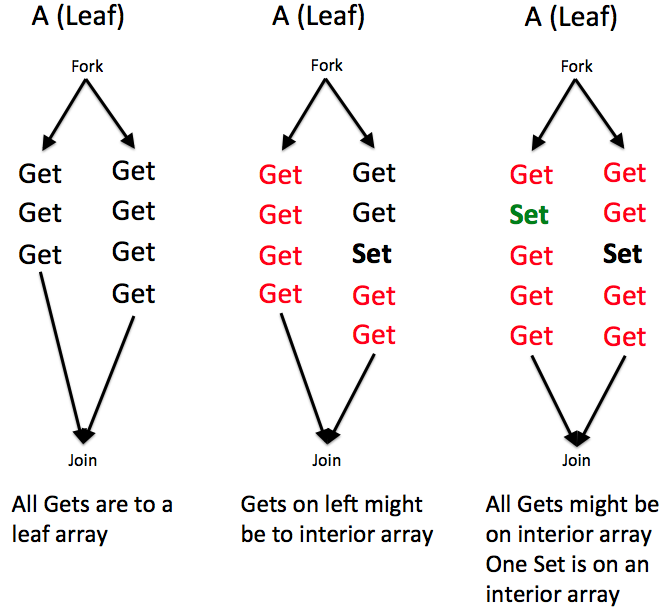
\includegraphics[scale=0.3]{fork_join_intuition}
\nocaptionrule \caption{Different ways an array might be used in a fork join}
\label{fig:fork_join_intuition}
\end{figure}

We cannot make any assumptions about how the instructions in different branches of a fork are interleaved, so we give the worst case time complexity over all possible interleavings. We first compute the work of each fork separately. Then for arrays that are used in both forks, we add additional work at the join point. To compute the additional work at the join point, we keep track of the number of gets that cost $O(1)$ on each side of the fork. If the array was modified on the other side of the fork, then the modification might have happened before the get, so we need to charge additional work for the get.

Our cost dynamics are defined by the following judgement, where $\delta$ is the store, $e$ is the expression, $\delta'$ is the new store, $v$ is the value returned by evaluating $e$, $w$ is the work, and $s$ is the span.
$$\delta; e \boldsymbol\Downarrow \delta'; v; w; s$$

We give the cost dynamics for arbitrary expressions in our language:

$$\frac{}{\delta; c \Downarrow \delta; c; 1; 1} \text{ (constants)}$$

$$\frac{\begin{gathered}\delta; e_1 \Downarrow \delta'; \lambda x . e; w_1 ; s_1 \;\;\; \delta'; e_2 \Downarrow \delta'';v; w_2 ; s_2 \;\;\; \\ \delta''; [v/x]e \Downarrow \delta'''; v'; w_3 ; s_3\end{gathered}}{\delta; e_1 \; e_2 \Downarrow \delta'''; v'; 1+w_1+w_2+w_3; 1+s_1+s_2+s_3} \text{ (func-app)}$$

$$\frac{\delta; e_1 \Downarrow \delta'; true; w_1; s_1 \;\;\; \delta'; e_2 \Downarrow \delta''; v; w_2; s_2}{\delta; \text{if } e_1 \text{ then } e_2 \text{ else } e_3 \Downarrow \delta''; v; 1+w_1+w_2; 1+s_1+s_2} \text{ (if-true)}$$

$$\frac{\delta; e_1 \Downarrow \delta'; false; w_1; s_1 \;\;\; \delta'; e_3 \Downarrow \delta''; v; w_2; s_2}{\delta; \text{if } e_1 \text{ then } e_2 \text{ else } e_3 \Downarrow \delta''; v; 1+w_1+w_2; 1+s_1+s_2} \text{ (if-false)}$$

Arrays are represented by $(l, V)$ where $l$ is a label that uniquely identifies the array, and $V$ contains the values in the array. $V[i]$ is the $i^{\text{th}}$ value in the array. If \set{} has been called on an array, the array is an interior array (represented by $-$), otherwise the array is a leaf array (represented by $+$). 

Array functions have different costs depending on whether the array is a leaf or interior array. We thread a store $\delta$ through each operation. $\delta$ maps array labels $l$ to $(+/-, c)$, where $c$ represents the number of cheap \get{}s on the array. $L(\delta)$ denotes the set of labels in the store $\delta$. Let $f(n)$ be the work of calling \get{} on an interior array of size $n$ and $g(n)$ be the work of calling \set{} on an interior array of size $n$.

The cost dynamics for the functions on a functional array of size $n$ are:
$$\frac{A = (l,V) \;\;\; i \text{ val} \;\;\; v \text{ val} \;\;\; \delta[l \mapsto (+, c)] \;\;\; l' \not\in L(\delta)}{\delta; \tset \; A \; i \; v \Downarrow \delta[l \mapsto (-, c), l' \mapsto (+, 0)]; (l', V[i \mapsto v]); 1; 1} \text{  (set-leaf)}$$

$$\frac{A = (l,V) \;\;\; i \text{ val} \;\;\; v \text{ val} \;\;\; \delta[l \mapsto (-, c)] \;\;\;  l' \not\in L(\delta)}{\delta; \tset \; A \; i \; v \Downarrow \delta[l' \mapsto (+, 0)]; (l', V[i \mapsto v]); g(n); 1} \text{  (set-interior)}$$

$$\frac{\begin{gathered}\delta; e_1 \Downarrow \delta_1; A; w_1; s_1 \;\;\; \delta_1; e_2 \Downarrow \delta_2; i; w_2; s_2 \;\;\; \\ \delta_2; e_3 \Downarrow \delta_3; v; w_3; s_3 \;\;\; \delta_3; \tset \; A \; i \; v \Downarrow \delta'; A'; w'; s' \end{gathered}}{\delta; \tset \; e_1 \; e_2 \; e_3 \Downarrow \delta'; A'; w_1+w_2+w_3+w'; s_1+s_2+s_3+s'} \text{ (set-eval)}$$  

$$\frac{A = (l,V) \;\;\; i \text{ val} \;\;\; \delta[l \mapsto (+, c)]}{\delta; \text{get} \; A \; i \Downarrow \delta[l \mapsto (+, c+1)]; V[i]; 1; 1} \text{  (get-leaf)}$$

$$\frac{A = (l,V) \;\;\; i \text{ val} \;\;\; \delta[l \mapsto (-, c)]}{\delta; \text{get} \; A \; i \Downarrow \delta; V[i]; f(n); 1} \text{  (get-interior)}$$

$$\frac{\begin{gathered}\delta; e_1 \Downarrow \delta_1; A; w_1; s_1 \;\;\; \delta_1; e_2 \Downarrow \delta_2; i; w_2; s_2 \;\;\; \\ \delta_2; \tget \; A \; i \Downarrow \delta'; v'; w'; s' \end{gathered}}{\delta; \tget \; A \; i \Downarrow \delta'; v'; w_1 + w_2 + w'; s_1 + s_2 + s'}\text{ (get-eval)}$$

$$\frac{\begin{gathered}\delta, e_L \Downarrow \delta_L; v_L; w_L, s_L \;\;\; \delta, e_R \Downarrow \delta_R; v_R; w_R, s_R \;\;\; \\ (L(\delta_L) \setminus L(\delta)) \cap (L(\delta_R) \setminus L(\delta)) = \emptyset\end{gathered}}{\delta; (e_L || e_R) \Downarrow \delta'; (v_L || v_R); 1 + w_L + w_R + w'; \max(s_L, s_R)} \text{  (fork-join)}$$

\set{} creates a new label and array and modifies the store to indicate that the newly created array is a leaf array, and the array \set{} was called on has become an interior array. The work for \set{} is higher for interior arrays. \get{} returns the value at the desired index, if the array is a leaf then the operation costs 1 unit of work but we increment the counter of cheap \get{}s in the store.

The fork-join cost semantics are the most interesting. Suppose we have an expression $e_L || e_R$ and
\[ \delta, e_L \Downarrow \delta_L; v_L; w_L, s_L \]
\[ \delta, e_R \Downarrow \delta_R; v_R; w_R, s_R \]

Further, suppose that $(\delta_L \setminus \delta) \cap (\delta_R \setminus \delta) = \emptyset$ (the new labels produced on both sides of the fork-join do not conflict). Consider an array $A = (l, V)$ with $\delta[l] = (s,c)$, $\delta_L[l] = (s_L, c + c_L)$, $\delta_R[l] = (s_R, c + c_R)$. When multiplying two signs or multiplying a sign with an integer, consider + to be 1 and - to be 0. 

\func{Combine} describes how to combine the values in the store on both sides of the fork-join. The array is a leaf array iff it is a leaf array on both sides of the fork-join. Cheap \get{}s on one side of the fork remain cheap iff there were no calls to \set{} on the other side of the fork.
\begin{equation*}
  \begin{aligned}
   \text{\func{combine}}&((s, c), (s_L, c + c_L), (s_R, c + c_R))= \\
   &(s_L s_R, c + s_R c_L + s_L c_R)
  \end{aligned}
\end{equation*}
$$\delta' = \; (\delta_L / \delta) \; \cup \; (\delta_R / \delta) \; \cup \bigcup_{l \in L(\delta)} [l \mapsto \text{\func{combine}}(\delta[l], \delta_L[l], \delta_R[l])]$$
\func{Extrawork} gives the additional cost incurred if an array of size $n$ was modified on either side of a fork-join. If the array was an interior array before the fork-join, then all functions incurred their maximal cost and there is no additional cost. Otherwise, cheap \get{}s on one side of the fork are charged $f(n)$ work iff the other side of the fork called \set{}. If both sides of the fork called \set{}, then one of the \set{}s came first and has work $1$, the subsequent \set{} has work $g(n)$.
\begin{equation*}
  \begin{aligned}
  \text{\func{extra}}&\text{\func{work}}(l, (s, c), (s_L, c + c_L), (s_R, c + c_R)) = \\
  & ((\neg s_R) c_L  + (\neg s_L) c_R)(f(size(l))-1) + \\
  &s(\neg s_R) (\neg s_L) (g(size(l))-1)
 \end{aligned}
\end{equation*}
$$w' = \sum_{l \in L(\delta), \delta[l \mapsto (+, c)]} \text{\func{extrawork}}(l, \delta[l], \delta_L[l], \delta_R[l])$$
Then, the fork-join cost semantics are:
$$\delta; (e_L || e_R) \Downarrow \delta'; (v_L || v_R); 1 + w_L + w_R + w'; \max(s_L, s_R)$$

\tabulate{} involves multiple function calls in parallel, so its cost semantics use \func{combine} and \func{extrawork} multiple times. We omit discussion of \tabulate{} here and in the rest of the paper because it involves messy details that are not relevant to the goals of this paper.

\section{Analysis}

\subsection{Interleaved Structural Dynamics}

To show that our implementation is correct and to validate our cost dynamics, we introduce interleaved structural dynamics for the source language. The structural dynamics describe the possible steps a program in our source language can take and are given by the following judgement, where $S$ is the store, $e$ is the expression, $S'$ is the resulting store, $e'$ is the resulting expression after a step has been taken, and $w$ is the work.

$$S, e \to S', e', w$$

For now we let the span of each step be 1 (we account for the spans later on).

As before, arrays are represented by $(l, V)$ where $l$ is a unique label and $V$ contains the values in the array. However, the store $S$ maps labels only to $+$ (leaf) or $-$ (interior). $L(S)$ denotes the set of labels in the store $S$. \func{size}$(l)$ denotes the size of the array referenced by label $l$. The judgement \func{val} describes terminal values. The structural dynamics are given as follows:
$$\frac{e_2 \; \text{val}}{S, (\lambda x.e)e_2 \to S, [e_2/x]e, 1} \text{ (app-sub)}$$
$$\frac{S, e_2 \to S', e_2', w}{S, (\lambda x.e) e_2 \to S', (\lambda x.e) e_2', w} \text{ (app-arg)}$$
$$\frac{S, e_1 \to S', e_1', w}{S, e_1 e_2 \to S', e_1' e_2, w} \text{ (app-func)}$$
$$\frac{}{S, \text{if } true \text{ then } e_2 \text{ else } e_3 \to S, e_2, 1} \text{ (if-true)}$$
$$\frac{}{S, \text{if } false \text{ then } e_2 \text{ else } e_3 \to S, e_3, 1}  \text{ (if-false)}$$
$$\frac{S, e_1 \to S', e_1', w}{S, \text{if } e_1 \text{ then } e_2 \text{ else } e_3 \to S', \text{if } e_1' \text{ then } e_2 \text{ else } e_3, w} \text{ (if-cond)}$$
$$\frac{A = (l, V) \;\;\; S[l] = + \;\;\; i \text{ val}}{S, get(A, i) \to S, V[i], 1} \text{ (get-leaf)}$$
$$\frac{A = (l, V) \;\;\; S[l] = -  \;\;\; i \text{ val}}{S, get(A, i) \to S, V[i], f(size(l))} \text{ (get-interior)}$$
$$\frac{A = (l, V) \;\;\; S, e_2 \to S', e_2', w}{S, get(A, e_2) \to S', get(A, e_2'), w} \text{ (get-index)}$$
$$\frac{S, e_1 \to S', e_1', w}{S, get(e_1, e_2) \to S', get(e_1', e_2), w} \text{ (get-array)}$$
$$\frac{A = (l, V) \;\;\; S[l] = + \;\;\;  l' \not\in L(S) \;\;\; i \text{ val} \;\;\; v \text{ val}}{S, set(A, i, v) \to S[l \mapsto -], (l', V[i \mapsto v]), 1} \text{ (set-leaf)}$$
$$\frac{A = (l, V) \;\;\; S[l] = - \;\;\;  l' \not\in L(S) \;\;\; i \text{ val} \;\;\; v \text{ val}}{S, set(A, i, v) \to S, (l', V[i \mapsto v]), g(size(l))} \text{ (set-interior)}$$
$$\frac{A = (l, V) \;\;\; i \text{ val} \;\;\; S, e_3 \to S', e_3', w}{S, set(A, i, e_3) \to S', set(A,i,e_3'), w} \text{ (set-val)}$$
$$\frac{A = (l, V) \;\;\; S, e_2 \to S', e_2', w}{S, set(A, e_2, e_3) \to S', set(A,e_2',e_3), w} \text{ (set-index)}$$
$$\frac{e_1 \to S', e_1', w}{S, set(e_1, e_2, e_3) \to S', set(e_1',e_2,e_3), w} \text{ (set-array)}$$

The structural dynamics for fork-join is non-deterministic since either side of the fork can take a step.
$$\frac{S, e_1 \to S', e_1', w}{S, e_1 || e_2 \to S', e_1' || e_2, w} \text{ (fork-left)}$$
$$\frac{S, e_2 \to S', e_2', w}{S, e_1 || e_2 \to S', e_1 || e_2', w} \text{ (fork-right)}$$

The structural dynamics for tabulate is also non-deterministic.

\begin{definition}
A \emph{transition sequence} $T$ is a sequence of states $[(S_0, e_0), ..., (S_n, e_n)]$ and costs $[w_1, ..., w_n]$ s.t. for all $0 \leq i < n$, $S_i, e_i \to S_{i+1}, e_{i+1}, w_{i+1}$ . We say that $T$ takes $S_0, e_0$ to $S_n, e_n$ and has length $n$ and denote this by $S_0, e_0 \to^n S_n, e_n$.
\end{definition}

\begin{definition}
We say that $T$ is \emph{maximal} if there does not exist $S', e', w'$ s.t. $S_n, e_n \to S', e', w'$.
\end{definition}

\begin{definition}
A \emph{transition subsequence} $T_{i, j}$ of $T$ is given by the sequence of states $[(S_i, e_i), ..., (S_j, e_j)]$ and costs $[w_{i+1}, ..., w_j]$. Note that $T = T_{0,n}$.
\end{definition}

\begin{definition}
The \emph{work of a transition sequence} $T$ is given by:
$$W(T) = \sum_{i=1}^n w_i$$
Different transition sequences starting and ending at the same states may have different work.
\end{definition}

\subsection{Sequential Cost Analysis}

\begin{definition}
Consider a transition sequence $T$. We say that $S_i, e_i \to S_{i+1}, e_{i+1}, w_{i+1}$ is a get on $l$ if the step involves evaluating the get function on array $(l, V)$. We say it is a \emph{cheap get} on $l$ if $w_{i+1} = 1$. The number of cheap gets on $l$ in $T$ is denoted by $SC_l(T)$.
\end{definition}

\begin{definition}
Unlike the store in the evaluational dynamics, the store in the structural dynamics only stores whether each array is $+$ (leaf) or $-$ (interior). $sign(\delta)$ takes a store that maps $l \mapsto (s,c)$ and returns a store which maps $l \mapsto s$.
\end{definition}

\begin{definition}
Suppose that $\delta, e \Downarrow \delta', e', w', s'$. We define the number of cheap gets in going from $\delta$ to $\delta'$ in the evaluational dynamics as follows. Suppose $l \mapsto (s', c') \in \delta'$. If $l \mapsto (s,c) \in \delta$ then $EC_l(\delta, \delta') = c' - c$ and if $l \not\in \delta$ then $EC_l(\delta, \delta') = c'$. If $l \not\in \delta'$ then $EC_l(\delta, \delta') = 0$.
\end{definition}

\begin{definition}
A \emph{relabeling} of $L_1$ is a bijective function $R$ from label sets $L_1 \to L_2$. $R$ can be used to relabel stores and expressions. $R(\delta) = \{ R(l) \mapsto e \; | \; l \mapsto e \in \delta \wedge l \in L_1  \} \cup \{ l \mapsto e \; | \; l \mapsto e \in \delta \wedge l \not\in L_1  \}$. In other words, $R$ relabels some of the labels in $\delta$. Similarly, $R(e)$ returns an expression $e'$ where each occurrence of a label $l$ in $e$ is substituted by $R(l)$.
\end{definition}

\begin{lemma}
\label{relabeling_lemma}
Suppose that there exists a derivation of length $m$ that $\delta, e \Downarrow \delta', e', w, s$. Let $R$ be an arbitrary labeling. Then there exists a derivation of length $m$ that $R(\delta), R(e) \Downarrow R(\delta'), R(e'), w, s$.
\end{lemma}

\begin{proof}
By applying the relabeling to each step of the derivation, and noting that all rules in the evaluational dynamics hold under relabelings.
\end{proof}

\begin{lemma}
\label{stateless_lemma}
If $S, e \to S', e', w$ and $U$ is a store s.t. for all $l \in e$, $l \in U$, then there exists $U', w'$ s.t. $U, e \to U', e', w'$
\end{lemma}

\begin{proof}
By casing on each rule in the structural dynamics, and noting that transitions of expressions never depend on the values in the store.
\end{proof}

\begin{theorem}
\label{main_work_theorem}
Suppose that 
$$\delta, e_0 \Downarrow \delta_E, e_E, w_E, s_E$$

and consider arbitrary maximal transition sequence T taking 
$$S_0 = sign(\delta), e_0 \to^n S_n, e_n$$
�
The following hold:
\begin{enumerate}
\item For some relabeling $R$ of $L(\delta_E) \setminus L(\delta)$, $S_n = sign(R(\delta_E))$ and $e_n = R(e_E)$.
\item For all $l \in \delta_E$, $EC_l(\delta, \delta_E) \leq SC_{R(l)}(T)$.
\item The sum of work and cheap gets is conserved: \begin{align*}
w_E + &\sum_{l \in L(\delta_E)} EC_l(\delta, \delta_E) (f(size(l))-1) =\\
 &W(T) + \sum_{l \in L(\delta_E)} SC_{R(l)}(T) (f(size(R(l))) - 1)
 \end{align*}
\end{enumerate}
\end{theorem}

\begin{proof}
By induction on the length of the shortest derivation in the evaluation dynamics. We prove the theorem for 2 of the rules in the evaluation dynamics: get-leaf and fork-join. The other cases follow from a similar line of reasoning.
\\

\noindent \textbf{Case get-leaf}: Suppose $e_0 = get(e_L, e_R)$ and
$$\delta, e_L \Downarrow \delta_L, e_L', w_L$$
$$\delta_L, e_R \Downarrow \delta_R, e_R', w_R$$
$$\delta_R, get(e_L', e_R') \Downarrow \delta_E, e_E, 1$$
which gives us
$$\delta, get(e_L, e_R) \Downarrow \delta_E, e_E, w_E$$
with $w_E = w_L + w_R + 1$.

Note that the structural dynamics first step the left argument to get, then the right argument, and finally evaluate the get. So there exists $m$ such that $T_{0,m}$ involves stepping the left argument, $T_{m,n-1}$ involves stepping the right argument, and $T_{n-1,n}$ involves evaluating the get.

\textbf{Part 1}: Suppose that in $T_{0,m}$, for $0 \leq i \leq m$, $e_i = get(e_{L,i}, e_R)$. Consider a new projected transition sequence $T_{0,m}'$ with states $[(S_0, e_{L,0}), ..., (S_m, e_{L,m})]$ and costs the same as $T_{0,m}$: $[w_1, ..., w_m]$. It is easy to verify that $T_{0,m}'$ is a valid transition sequence starting at $(S_0, e_{L,0})$ and is maximal. 

$S_0 = sign(\delta)$ and $e_{L,0} = e_L$ so we can apply the IH to $T_{0,m}'$. For some relabeling $R$ of labels in $L(\delta_L) / \delta$, $s_m = sign(R(\delta_L))$ and $e_{L,m} = R(e_L')$ $\Rightarrow$ $e_m' = (e_{L,m}, e_R) = (R(e_L'), e_R)$. WLOG suppose that $\delta_L$ was labeled such that the above hold (we can do this because of lemma \ref{relabeling_lemma}). Note that in subsequent parts of the proof, we omit creating the projected transition sequence and apply the IH directly to $T_{0,m}$ when needed.

Using similar logic on $T_{m,n-1}$ we get that for some relabeling of $\delta_R / \delta_L$, applying that relabeling to $\delta_R$ and $(e_L', e_R')$ gives us $e_{n-1} = (e_L', e_R')$ and $S_{n-1} = sign(\delta_R)$. WLOG suppose that $\delta_R$ was labeled so that the above holds.

By combining the relabelings of $\delta_L / \delta$ and $\delta_R / \delta_L$ and applying that to $(e_L', e_R')$ and $\delta_R$, we get that $e_{n-1} = get(e_L', e_R')$ and $S_{n-1} = sign(\delta_R)$. Note that get does not change the sign of any label in the store in either the structural or the evaluation dynamics, so $sign(\delta_E) = sign(\delta_R) = S_{n-1} = S_n$. Further, the structural and evaluational dynamics apply get in the same way, so $e_n = e_E$. Therefore the first part of this theorem holds. WLOG suppose that the stores and expressions were relabeled s.t. the first part holds.

\textbf{Part 2}: From lemma \ref{relabeling_lemma}, the length of the shortest derivation for the relabeled evaluational dynamics does not change, so we can apply the inductive hypothesis. Applying the IH to $T_{0,m}$, for all $l \in \delta_L$, $EC_l(\delta, \delta_L) \leq SC_l(T_{0,m}') = SC_l(T_{0,m})$. If $l \in \delta_R$ but $l \not\in \delta_L$ then $EC_l(\delta, \delta_L) = SC_l(T_{0,m}) = 0$ (intuitively the label did not exist and so did not have any cheap gets), so in particular, for all $l \in \delta_R$, $EC_l(\delta, \delta_L) \leq SC_l(T_{0,m})$. Applying the IH to $T_{m,n-1}$ we get that for all $l \in \delta_R$, $EC_l(\delta_L, \delta_R) \leq SC(T_{m,n-1})$.

We note that $EC$ and $SC$ are additive, that is,
$$EC_l(\delta, \delta_R) = EC_l(\delta, \delta_L) + EC_l(\delta_L, \delta_R)$$
$$SC_l(T_{0,n-1}) = SC_l(T_{0,m}) + SC_l(T_{m,n-1})$$
This implies that for all $l \in \delta_R$, $EC_l(\delta, \delta_R) \leq SC_l(T_{0,n-1})$. 

Now, let $e_L' = (l',V)$ with $l' \in \delta_R$. Then, $EC_{l'}(\delta, \delta_E) = EC_{l'}(\delta, \delta_R) + 1$ and $SC_{l'}(T) = SC_{l'}(T_{0,n-1}) + 1$, so $EC_{l'}(\delta, \delta_E) \leq SC_{l'}(T)$. If $l \neq l'$ then $EC_{l}(\delta, \delta_E) = EC_{l}(\delta, \delta_R)$ and $SC_{l}(T) = SC_{l}(T_{0,n-1})$, so $EC_{l}(\delta, \delta_E) \leq SC_{l}(T)$. So the second part of the theorem holds.

\textbf{Part 3}: The third part of the theorem follows by similarly applying the IH on $T_{0,m}$ and $T_{m,n-1}$, and noting that $W(T) = W(T_{0,m}) + W(T_{m,n-1}) + 1$.
\\

\noindent \textbf{Case fork-join}: Suppose $e_0 = (e_L || e_R)$ and
$$\delta, e_L \Downarrow \delta_L, v_L, w_L$$
$$\delta, e_R \Downarrow \delta_R, v_R, w_R$$
which gives us
$$\delta, (e_L || e_R) \Downarrow \delta', (v_1 || v_2), 1 + w_L + w_R + w'$$
with $w'$ and $\delta'$ defined in terms of \func{extrawork} and \func{combine} as given in the evaluational dynamics.

In T, for all $0 \leq i \leq n$ let $e_i = (e^L_i || e^R_i)$. Let $I_L$ be the sequence of all $0 \leq i \leq n-1$ where transitioning from $e_i$ to $e_{i+1}$ involved stepping the left argument. Let $m$ be the length of $I_L$. Similarly define $I_R$ for the right argument, and let $k$ be the length of $I_R$.

Let $A$ be the sequence of $e^L$s corresponding the indices in $I_L$, and add $e^L_n$ at the end of $A$. Similarly, let $B$ be the sequence of $e^R$s corresponding the indices in $I_R$, adding $e^R_n$ at the end.

Let $S^L_0 = S_0 = sign(\delta)$. By inductively applying lemma \ref{stateless_lemma}, there exists $S^L_1, ... S^L_m$ s.t. $T_L = [(S^L_0, A_0), ..., (S^L_m, A_m)]$ is a transition sequence. $T_L$ is maximal, because if $A_m$ in $T_L$ can take a step then $e^L_n$ in $T$ can take the corresponding step. Similarly, let  $S^R_0 = S_0 = sign(\delta)$. Then, there exists $S^R_1, ... S^R_k$ s.t. $T_R = [(S^R_0, B_0), ..., (S^R_k, B_k)]$ is a maximal transition sequence.

Applying the IH on $T_L$, we get a relabeling $R_L$ on $L(\delta_L) \setminus L(\delta)$ s.t. $R_L(v_L) = A_m = e^L_n$ and $sign(R_L(\delta_L)) = S^L_m$. Similarly, we get a relabeling $R_R$ on $L(\delta_R) \setminus L(\delta)$ s.t. $R_R(v_R) = B_k = e^R_n$ and $sign(R_R(\delta_R)) = S^R_k$. 

By inducting on the product $mk$, we can show that the new labels produced in $T_L$ and $T_R$ do not overlap, that is: $(L(S^L_m) \setminus L(S_0)) \cap (L(S^R_k) \setminus L(S_0)) = \emptyset$. (Note to self: Should I sketch out this induction?). Compose the relabelings to get relabeling R.

Applying lemma $\ref{relabeling_lemma}$ and the fork join rule, we get,
$$\delta, R(e_L) \Downarrow R(\delta_L), R(v_L), w_L$$
$$\delta, R(e_R) \Downarrow R(\delta_R), R(v_R), w_R$$
which gives us
$$\delta, R((e_L || e_R)) \Downarrow R(\delta'), R((v_1 || v_2)), 1 + w_L + w_R + w'$$

with $R((v_1||v_2)) = (R(v_1) || R(v_2)) = (e_n^L || e_n^R)$. To reduce clutter, WLOG suppose that the stores and expressions in the evaluational dynamics were labeled as such. By lemma \ref{relabeling_lemma} we can apply the IH on the relabeled evaluational dynamics since the length of the shortest derivation is invariant under relabelings.

\begin{lemma}
\label{label_projection_lemma}
$l \in S_n$ if and only if either $l \in S^L_m$ or $l \in S^R_k$
\end{lemma}

\begin{proof}
If $l \in S_0$ the claim holds trivially. Otherwise,

$(\Rightarrow)$ By considering the step in $T$ that first introduced $l$, and examining the corresponding step in either $T_L$ or $T_R$.

$(\Leftarrow)$ By considering the step in $T_L$ (or $T_R$) that first introduced $l$ and examining the corresponding step in $T$.
\end{proof}

\begin{lemma}
\label{sign_projection_lemma}
$S_n[l] = -$ if and only if either $l \in S^L_m$ and $S^L_m[l] = -$ or $l \in S^R_k$ and $S^R_k[l] = -$
\end{lemma}

\begin{proof}
Similar to lemma \ref{label_projection_lemma}.
\end{proof}

\textbf{Part 1}: We claim that the set of labels in $\delta'$ and $S_n$ are the same. From the evaluational dynamics, $L(\delta') = L(\delta_L) \cup L(\delta_R)$. Since $sign(\delta_L) = S^L_m$ and $sign(\delta_R) = S^R_k$, $L(\delta_L) = L(S^L_m)$ and $L(\delta_R) = L(S^R_k)$. From lemma $\ref{label_projection_lemma}$, $L(S_n) = L(S^L_m) \cup L(S^R_k) = L(\delta')$ which proves the claim. 

To show that $sign(\delta') = S_n$ we case on arbitrary $l \in L(\delta')$ and show that $sign(\delta')[l] = S_n[l]$:

\textbf{Case $l \in L(\delta)$}: 

If $\delta[l] = (-,\_)$ then $S_0[l] = -$. The evaluational and structural dynamics do not change $-$ to $+$ so $\delta'[l] = (-,\_)$ and $S_n[l] = -$ so $sign(\delta')[l] = S_n[l]$.

Suppose $\delta[l] = (+, \textunderscore)$, in which case $S_0[l] = +$. If $\delta'[l] = (+,\_)$, then from the way combine works, $\delta_L[l] = (+, \_)$ and $\delta_R[l] = (+, \_)$. From the IH $S^L_m[l] = +$ and $S^R_k[l] = +$. From lemma \ref{sign_projection_lemma} $S_n[l] = + = sign(\delta')[l]$. 

On the other hand, if $\delta[l] = (+, \textunderscore)$ (in which case $S_0[l] = +$) but $\delta'[l] = (-,\_)$, then from the way combine works, either $\delta_L[l] = (-,\_)$ or $\delta_R[l] = (-, \_)$. WLOG suppose that $\delta_L[l] = (-,\_)$. From the IH, $S^L_m[l] = -$. From lemma \ref{sign_projection_lemma} $S_n[l] = - = sign(\delta')[l]$.

\textbf{Case $l \in L(\delta_L), l \not\in L(\delta)$}: Then $l \not\in \delta_R$ so $\delta'[l] = \delta_L[l]$. From IH, $sign(\delta_L) = S^L_m$. Since $l \not\in \delta_R$, $l \not\in S^R_k$ so by applying lemma \ref{sign_projection_lemma}, $S^L_m[l] = S_n[l]$, as desired.

The case where $l \in L(\delta_R), l \not\in L(\delta)$ is symmetric.

Finally, we note that $(v_1||v_2) = (e^L_n||e^R_n)$ from the way $v_1,v_2$ were relabeled.

\textbf{Part 2}: 

We case on arbitrary $l \in \delta'$.

\textbf{Case $l \in L(\delta)$}: 

If $\delta[l] = (-,c)$ then $EC_l(\delta, \delta') = 0 = SC_l(T)$.

Else suppose $\delta_L[l] = (+,c_1)$ and $\delta_R[l] = (+,c_2)$. Then $SC_l(T) = SC_l(T_L) + SC_l(T_R) \geq EC_l(\delta, \delta_L) + EC_l(\delta, \delta_R) = EC_l(\delta, \delta')$.

Else suppose $\delta_L[l] = (+,c_1)$ and $\delta_R[l] = (-,c_2)$. We can show that all the cheap \get{}s in $T_R$ are cheap in $T$. So $SC_l(T) \geq SC_l(T_R) \geq EC_l(\delta, \delta_R) = EC_l(\delta, \delta)$.

The case where $\delta_L[l] = (-,c_1)$ and $\delta_R[l] = (+,c_2)$ follows by symmetry.

Finally, if $\delta_L[l] = (-,c_1)$ and $\delta_R[l] = (-,c_2)$, then $SC_l(T) \geq 0 = EC_l(\delta, \delta')$.

\textbf{Case $l \in L(\delta_L), l \not\in L(\delta)$} Then $EC_l(\delta, \delta') = EC_l(\delta, \delta_L)$ since $l \not\in \delta_R$. By IH, $EC_l(\delta, \delta_L) \leq SC_l(S_0, S^L_m)$. Since $l \not\in S^R_k$, $SC_l(S_0, S^L_m) = SC_l(S_0, S_n)$ and so the claim holds.

The case where $l \in L(\delta_R), l \not\in L(\delta)$ is similar.

\textbf{Part 3:} We omit the formal proof of this part because it contains tedious algebraic details but the key ideas are described below.

In the conservation expression, each \get{} on each array $(l,V)$ in both the evaluational and structural dynamics is charged $f(size(l))$. In particular, note that we add an additional $f(size(l))-1$ cost for cheap \get{}s that were charged 1 unit of work. Since the number of \get{}s is the same, the total cost of \get{}s is the same in both dynamics.

The number of \set{}s that are charged $g(size(l))$ is the same for both the evaluational and structural dynamics. This can be shown by casing on the signs of the array on both sides of the fork. If and only if \set{} was called on an array on both sides of the fork, one of the \set{}s will cost $g(size(l))$. Since the number of \set{}s is the same, the total cost of \set{}s is the same in both dynamics.
\end{proof}

\begin{theorem}
(Work Bound) Given the conditions in theorem \ref{main_work_theorem}, $w_E \geq W(T)$
\end{theorem}

\begin{proof}
We assume that $\delta_E$ has been relabeled as described in part 1 of theorem \ref{main_work_theorem}. For all $l \in \delta_E$, $EC_l(\delta, \delta_E) \leq SC_l(T)$. This implies that $\displaystyle \sum_{l \in \delta_E} EC_l(\delta, \delta_E) (f(size(l))-1) \leq \sum_{l \in \delta_E} SC_l(T) (f(size(l))-1)$. But then from the conservation of sum of work and cheap gets, $w_E \geq W(T)$.
\end{proof}

\begin{theorem}
(Existence) Suppose that $\delta, e_0 \Downarrow \delta_E, e_E, w_E, s_E$. Then, for some $n$, there exists a transition sequence $T$ from $s_0 = sign(\delta), e_0 \to^n s_n, e_n$.
\end{theorem}

\begin{proof}
We can construct such a transition sequence $T$ inductively, by inducting on the rules of the evaluational dynamics.
\end{proof}

\begin{theorem}
(Termination) Suppose that $\delta, e_0 \Downarrow \delta_E, e_E, w_E, s_E$. Then there exists $n$ s.t. all transition sequences starting at $sign(\delta), e_0$ have length $\leq n$.
\end{theorem}

\begin{proof}
By induction on the rules of the evaluational dynamics.
\end{proof}

When evaluating an expression $e$ in our language, the stores are initially empty. In particular, the signs of the store in the evaluational dynamics and structural dynamics are the same. From the existence theorem, we know there exists a transition sequence $T$ starting at $e$. From the termination theorem, all transition sequences starting at $e$ have bounded length. Then, from the work bound theorem, we get that the work computed by the evaluational dynamics is more than the work of any transition sequence. Since the structural dynamics captures the (non-deterministic) execution time of the expression, this means that the evaluational dynamics overestimates the execution time of the expression.

\subsection{Parallel Structural Dynamics}

The parallel dynamics are given by the following judgement, where $e$ is the expression and $e'$ is the resulting expression:
$$e \to_{par} e'$$
The parallel dynamics represent the evaluation steps taken on a machine with infinite processors. We show the dynamics for get and fork-join.
$$\frac{A \; \text{val} \;\;\; i \; \text{val}}{\tget{} \; A \; i \to_{par} A[i]} \text{ (get)}$$
$$\frac{A \; \text{val} \;\;\; e_2 \to_{par} e_2'}{\tget{} \; e_1 \; e_2 \to_{par} \tget{} \; e_1 \; e_2'} \text{ (get-index)}$$
$$\frac{e_1 \to_{par} e_1'}{\tget{} \; e_1 \; e_2 \to_{par} \tget{} \; e_1' \; e_2} \text{ (get-array)}$$
$$\frac{e_1 \to_{par} e_1' \;\;\; e_2 \to_{par} e_2'}{e_1 || e_2 \to_{par} e_1' || e_2'} \text{ (fork-join)}$$
$$\frac{v_1 \; \text{val} \;\;\; e_2 \to_{par} e_2'}{v_1 || e_2 \to_{par} v_1 || e_2'} \text{ (fork-join-right)}$$
$$\frac{v_2 \; \text{val} \;\;\; e_1 \to_{par} e_1'}{e_1 || v_2 \to_{par} e_1' || v_2} \text{ (fork-join-left)}$$

Notice that in fork-join, both sides of the fork-join take a step at the same time if possible. The other rules are similar to the rules for get. The parallel structural dynamics, unlike the sequential structural dynamics, are deterministic. 

A parallel transition sequence $T$ is a sequence $(e_0, ..., e_n)$ with $e_i \to_{par} e_{i+1}$ for all $0 \leq i < n$. We say that $e_0 \to^n_{par} e_n$. The span of $T$, denoted by $SP(T)$, is its length $n$. The span represents the number of steps taken to evaluate an expression on a machine with an unbounded number of processors.

\subsection{Parallel Cost Analysis}

\begin{theorem}
Suppose that 
$$\delta, e_0 \Downarrow \delta_E, e_E, w_E, s_E$$
and consider arbitrary parallel transition sequence $T$ taking
$$e_0 \to^n_{par} e_n$$
Then $SP(T) \leq s_E$
\end{theorem}

\begin{proof}
By induction on the rules of the evaluational dynamics. We prove the theorem for 2 of the rules in the evaluational dynamics: get and fork-join. The other cases follow from a similar line of reasoning.
\\

\noindent \textbf{Case get:} Suppose $e_0 = get(e_L, e_R)$ and
$$\delta, e_L \Downarrow \delta_L, e_L', w_L, s_L$$
$$\delta_L, e_R \Downarrow \delta_R, e_R', w_R, s_R$$
$$\delta_R, get(e_L', e_R') \Downarrow \delta_E, e_E, 1, 1$$
which gives us
$$\delta, get(e_L, e_R) \Downarrow \delta_E, e_E, w_E, s_E$$
with $s_E = s_L + s_R + 1$.

The parallel structural dynamics first step the left argument to get, then the right argument, and finally evaluate the get. So we can split the parallel transition sequence $T$ into corresponding subsequences $T_L$, $T_R$, $T_g$. By the inductive hypothesis, $SP(T_L) \leq s_L$ and $SP(T_R) \leq s_R$. Also, $SP(T_g) = 1$. So $SP(T) = SP(T_L) + SP(T_R) + SP(T_g) \leq s_L + s_R + 1 = s_E$, and the claim holds.
\\

\noindent \textbf{Case fork-join}: Suppose $e_0 = (e_L || e_R)$ and
$$\delta, e_L \Downarrow \delta_L, v_L, w_L, s_L$$
$$\delta, e_R \Downarrow \delta_R, v_R, w_R, s_R$$
which gives us
$$\delta, (e_L || e_R) \Downarrow \delta', (v_1 || v_2), 1 + w_L + w_R + w', max(s_L, s_R)$$

We can split the parallel transition sequence $T$ into two sub-sequences, $T_1$ where both sides of the fork-join take a step, and $T_2$ where only one side of the fork-join takes a step. We can project $T$ to a transition sequence $T_L$ for the left side of the fork-join  and a transition sequence $T_R$ for the right side of the fork-join. From the IH, $SP(T_L) \leq s_L$ and $SP(T_R) \leq s_R$. Then, $SP(T) \leq max(SP(T_L), SP(T_R)) \leq max(s_L, s_R) = s_E$, so the claim holds.
\end{proof}

The above theorem shows that the span in the evaluational dynamics is an upper bound for the span in the parallel structural dynamics.

In reality, each step in our parallel structural dynamics could take up to $\log{N}$ steps when run on a machine with an unbounded number of processors (where N is the size of the array being operated on). Note that if an expression includes an array of size $N$, the array must have been created. Creating an array of size $N$ has work at least $N$, so $N \leq W$. This means that the time taken to evaluate $e$ on a machine with an unbounded number of processors is $\leq s_E \log{W}$.

(Explain what Brent's theorem says) By applying Brent's theorem, we get that on a $p$ processor machine, the number of steps taken to evaluate an expression is $\leq \frac{W}{p} + s_E \log{W}$.

\newpage

\subsection{Correctness}

(\textbf{Note: Everything from this point is going to be very significantly changed in the near future})

A formal proof of correctness involves many steps, some of which are orthogonal to the goals of this paper. We give an outline of what is needed to prove that our array implementation is correct, and show the important parts of the proof.

Step 1: First, we need to define an imperative target language and a target machine that supports concurrent memory accesses. We need to give an implementation of arrays that deals with concurrency issues. In the implementation, the execution of functions on the same array might overlap, so we prove that the implementation is linearizable. Linearizability allows us to assume that array functions happen atomically. We give a (not formal) sketch of this in a later section.

Step 2: With atomicity, the target language is equivalent to an intermediate language where array operations happen in a single step, but have the same effect as in the target language. Like in the source language, the structural dynamics for fork-join in the intermediate language will be non-deterministic.

Step 3: Finally, we need to show that an expression $e$ in the source language, and the compiled expression $e_I$ in the intermediate language will evaluate to the same value. This involves setting up a relation that describes when an expression $e$ in the source language and $e_I$ in the intermediate language are equivalent. Suppose $e_I \to e_I'$. We need to show that $\exists e'$ s.t. $e \to e'$ and $e'$ and $e_I'$ are equivalent. Since the value $e$ in the source language evaluates to is independent of the steps it takes, we can use induction to show that $e$ and $e_I$ evaluate to the same terminal value.

The core part of steps 2 and 3 is showing sequential correctness of functional arrays. We define a data structure invariant, show that it is maintained by all array functions, and show that this implies that all calls to get return the value that they should.

\begin{definition}
Consider an array $A_I$ in the implementation and an array $A$ in the source language. We say that $A_I ~ A$ if the following holds. Consider arbitrary index $i$ and suppose that $A[i]$ has value $val$. Suppose that $A_I$ has version $V$ and is pointing to an ArrayData object $AD$. If there exists some version in $AD.logs[i]$ which is greater than $V$ then there exists a log entry $(v', val)$ where $v'$ is the smallest version in $AD.logs[i]$ that is $\geq V$. If no version in $AD.logs[i]$ is greater than $V$, then $AD.values[i]$ is val.
\end{definition}

\begin{theorem}
Assuming that $f(1), ...f(n)$ evaluates to the same value in the source and implementation, $\text{tabulate}(f, n)$ evaluates to equivalent arrays in the source and implementation.
\end{theorem}

\begin{proof}
\end{proof}

\begin{theorem}
Suppose that $A_I$ in the implementation and $A$ in the source are equivalent. Then $get(A,i)$ in the source and $get(A_I, i)$ in the implementation returns the same value.
\end{theorem}

\begin{proof}
\end{proof}

\begin{theorem}
Suppose we have arrays $A_1, A_2, ..., A_m$ in the source and $B_1, B2, ..., B_m$ in the implementation with $A_i ~ B_i$ for all $i$. Suppose we execute $set(A_m, i, v)$ by $A$ and $set(B_m, i, v)$ by $B$. Then after executing the sets, $A_i ~ B_i$ for all $i$ and $A ~ B$.
\end{theorem}

\begin{proof}
\end{proof}

\section{Approach}

An array $A$ is a leaf array if the set function has not been called with $A$ as an argument, otherwise $A$ is an interior array. While the dynamics of our arrays are functional, the implementation is different for interior and leaf arrays. 

\begin{figure}[!ht]
\centering
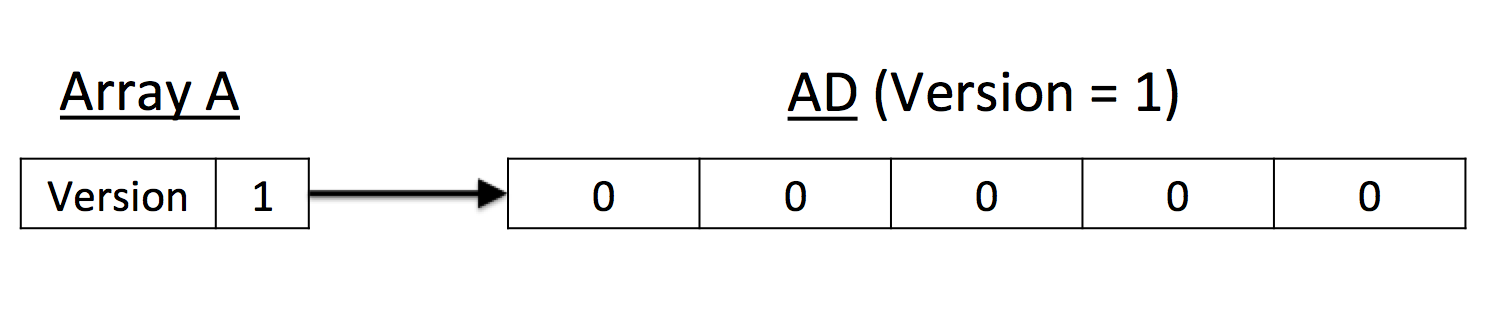
\includegraphics[scale=0.3]{new_array_A}
\nocaptionrule \caption{New functional array filled with 0s}
\label{fig:new_array_A}
\end{figure}

Suppose that $A$ is a leaf array  (see figure \ref{fig:new_array_A}). $A$ has a version number $V$, and a pointer to an ArrayData object $AD$. $AD$ keeps a regular (mutable) array of values, which corresponds to the values in $A$. $AD$ has a version number, which is the same as $A'$s ($V$) to indicate that $A$ is NEW. For each element of the array in $AD$, keep a log of values that used to be at that index. The logs are initially empty.

Get on leaf arrays: to get the $i^{\text{th}}$ element in $A$, simply access array[i] in $AD$.

\begin{figure}[!ht]
\centering
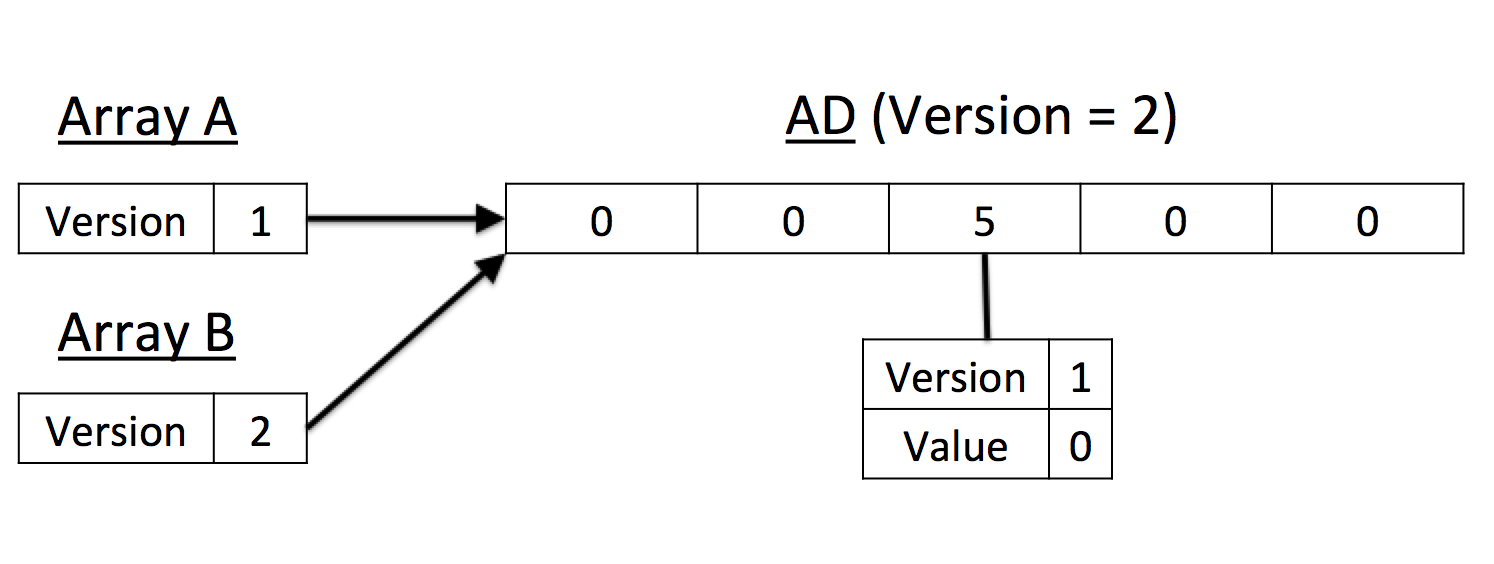
\includegraphics[scale=0.3]{set_A_return_B}
\nocaptionrule \caption{$B = set(A, 3, 5)$ changes the array in $AD$ and adds a log entry.}
\label{fig:set_A_return_B}
\end{figure}

Set on leaf arrays: Suppose that $A[i]$ is $v_{old}$ and we want to do $B = set(A, i, v_{new})$ (see figure \ref{fig:set_A_return_B}). Add an entry $(V, v_{old})$ to the log at index $i$, expressing that $A[i]$ was $v_{old}$ at version $V$. Increment the version of $AD$ to $V+1$. Set $array[i]$ in $AD$ to $v_{new}$. Create a new functional array $B$, with version $V+1$, which points to $AD$. Notice that both $A$ and $B$ point to $AD$. However, the version of $A$ is $V$ and the version of $AD$ is $V+1$, which indicates that $A$ is an interior array. The version of $B$ is $V+1$ which indicates that $B$ is NEW.

Get on interior array: Suppose we do $get(A, i)$ where $A$ is interior and has version $V$. We binary search the log at index $i$ to find what value was stored in the array at version $V$.

\begin{figure}[!ht]
\centering
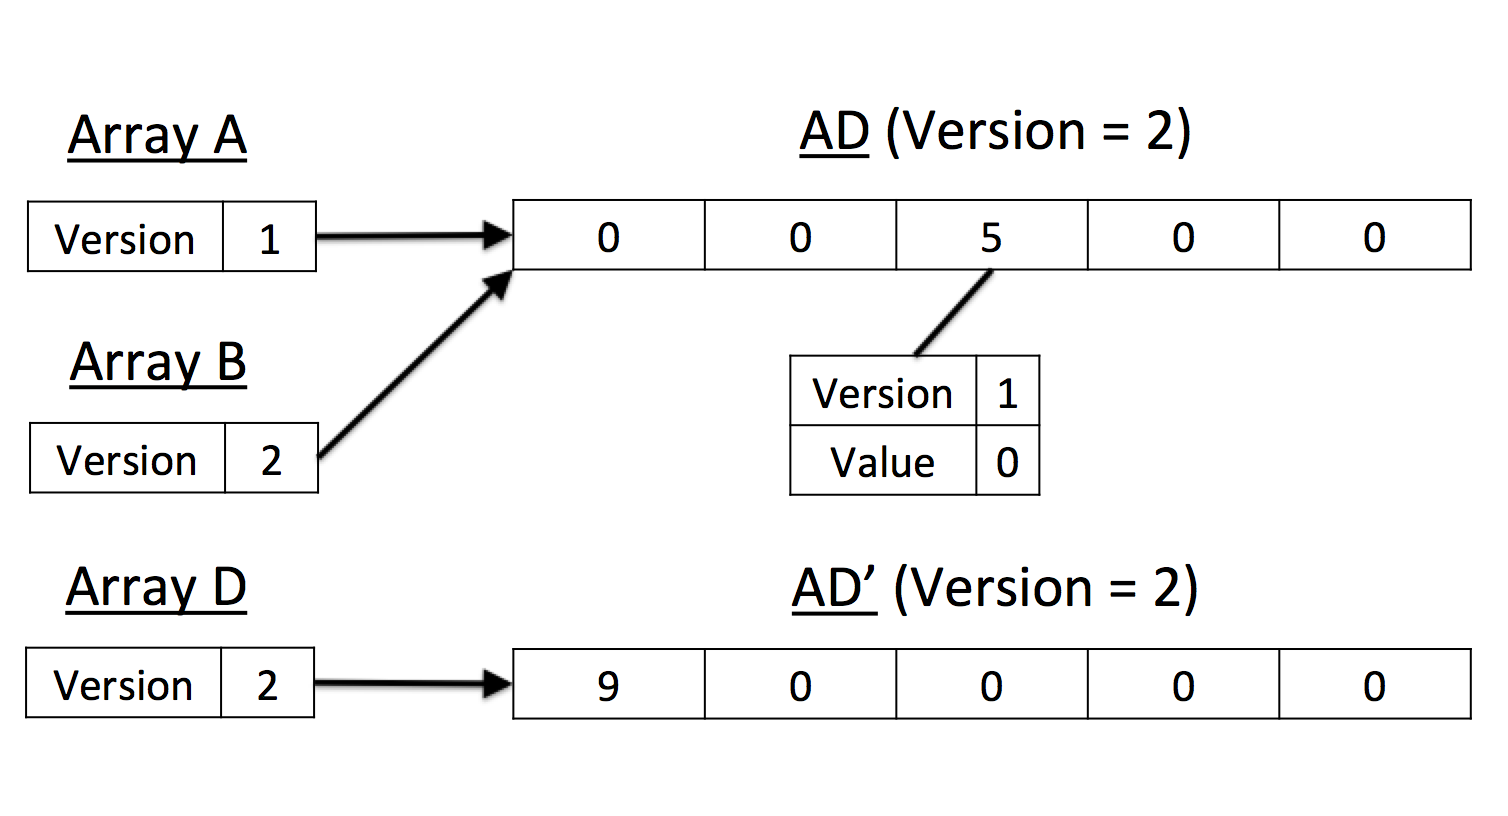
\includegraphics[scale=0.3]{set_old_array}
\nocaptionrule \caption{$D = set(A, 1, 9)$ copies $AD$ because $A$ is OLD}
\label{fig:set_old_array}
\end{figure}

Suppose we do $D = set(A, i,v)$ where $A$ is interior (see figure \ref{fig:set_old_array}). Create a new ArrayData object $AD'$ (with a new array). Copy the values from the array in $AD$ to the array in $AD'$, and then set $array[i]$ to $v$ in $AD'$.

The logs are stored in a doubling array which doubles in size when full. This guarantees amortized $O(1)$ insertion of a log entry, and allows us to binary search with $O(\log{m})$ work, where $m$ is the number of log entries.

Suppose that the size of the array is $n$. Every $n$ times an ArrayData object is modified, we create a new ArrayData object, and copy the values over to the new ArrayData object. This ensures that $m \leq n$ i.e. we don't have too many log entries in an ArrayData object. Copying is amortized $O(1)$.

It follows that in the RAM model the work of set and get is $O(1)$ for a leaf arrays. Get in an OLD array involves a binary search and has work $O(\log{n})$. Set in an OLD array involves copying the array, and has work $O(n)$.

\section{Concurrent Implementation}

We implement the functional array functions using an imperative target language.

\subsection{Concurrency Model}

We assume a sequential consistency model of concurrency. That is, when analyzing the effects of a program, we assume that at each time step exactly one pending instruction is executed. Consider the execution of a program $P$. We label the time steps in the execution from 1 to $t$. 

\begin{definition}
Consider an object $A$. Suppose that the program invokes functions $M_1$, $M_2$, ..., $M_n$ on $A$. Consider arbitrary $i$, and suppose that the instructions in $M_i$ were executed at times $s_1$, $s_2$, ..., $s_m$. We say that $A$ is \emph{linearizable} if the effect of the program is as if $M_i$ executed atomically at some time $s_j$, and this holds for all $M_i$.
\end{definition}

\begin{definition}
Suppose that first instruction in function call $f$ was executed at time $s_1$ and the last instruction at time $e_1$. Suppose that first instruction in function call $g$ was executed at time $s_2$ and the last instruction at time $e_2$. We say the function calls do not \emph{overlap} if the intervals $[s_1, e_1]$ and $[s_2, e_2]$ do not overlap.
\end{definition} 

Our programs have access to the link load store conditional (LLSC) function. LLSC takes an (address, old value, new value) tuple as argument. LLSC first checks that the value at address is the same as old value, if it is different then LLSC returns false. Otherwise LLSC atomically stores new value at address and returns true, however if the value at address was modified between the load and store, LLSC returns false.

\subsection{Push Arrays}

We use an auxiliary data structure, \emph{PushArrays}, to store log entries. PushArrays are initially empty and support 3 functions. Suppose we have a PushArray $A$. $A.push(e)$ inserts entry $e$, $A.size()$ returns the number of entries inserted, $A.get(i)$ returns the $i^{\text{th}}$ entry inserted. Note that $get$ is only defined between indices 0 and $A.size()-1$. All operations are amortized $O(1)$.

PushArrays can be used semi-concurrently. At most one thread can execute $push$ at any time, but multiple threads can call $size$ and $get$. In a PushArray $A$, $A.size$ stores the number of entries and $A.data$ references an array that stores the actual entries. Pseudocode for $A.push(e)$ is shown below.

\begin{lstlisting}[language=Java]
if (isFull(A.data)) {
  newData = new Array(A.data.capacity * 2);
  copyValues(from = A.data, to = newData);
  A.data = newData;
}
A.data[A.size] = e;
A.size += 1;
\end{lstlisting}

\begin{theorem}
Given that different calls to push (on the same PushArray) do not overlap, PushArrays are linearizable.
\end{theorem}

\begin{proof}
The linearization point of $push$ is $A.size$ $+=$ $1$, and the linearization point of the other functions is their single instruction. In push, expanding the capacity of $A.data$ when it is full does not interfere with accessing $A.data$ because we copy values to the new array before pointing $A.data$ to the new array. The effects of adding $e$ are only observable after we increase $size$, since, by the specification of PushArrays, the result of calling $A.get(i)$ where $i \geq A.size()$ is not defined.
\end{proof}

\subsection{Functional Array Implementation}

Suppose we have a FunctionalArray $A$. $A$ points to an ArrayData object which is referenced by $A.data$. The (imperative) array in $A.data$ is referenced by $A.data.values$, and the log entries corresponding to the $i^{\text{th}}$ index are stored in a PushArray $A.data.undo\_lists[i]$. We first explain the implementation of $A.set(pos, val)$.

We use a link load store conditional to ensure that only 1 thread can modify an ArrayData object at any time. If $m$ threads try to modify $A.data$, then $m-1$ threads will fail the LLSC (returning false). Instead of modifying $A.data$, these threads will create a new ArrayData object, and will copy over values from $A.data$, as shown below.

\begin{lstlisting}[language=Java]
FunctionalArray newA;
newA.version = A.version + 1;
if (!LLSC(&A.data.version, A.version, 
	newA.version) OR
    A.version % A.size == 0) {
  // Create a new ArrayData object AD
  // Forall i = 1:n, AD.values[i] = get(A, i)
  AD.values[pos] = val;
  newA.data = AD;
  return newA;
}
\end{lstlisting}

At most one of the threads trying to modify the ArrayData object will get past the LLSC, will insert a log entry and then modify $A.data.values$. The ordering of inserting a log entry and modifying $A.data.values$ matters in the proof of get. The pseudocode for this step is shown below.

\begin{lstlisting}[language=Java]
newA.data = A.data;
old_value = newA.data.values[pos];
undo_list = newA.data.undo_lists[pos];
undo_list.push((A.version, old_value));
newA.data.values[pos] = val;
return newA;
\end{lstlisting}

Next we explain the implementation of $A.get(pos)$.

\begin{lstlisting}[language=Java]
guess_val = A.data.values[pos];
if (A.version == A.data.version) {
  return guess_val;
}

undo_list = this.data.undo_lists[pos];
if (undo_list.size() == 0) {
  return guess_val;
}

upper = undo_list.size() - 1;
if (undo_list[upper].version < A.version) {
  return guess_val;
}
\end{lstlisting}

The last step is to binary search $undo\_list$, between the indices 0 and $upper$ (inclusive of 0 and upper). We find the log entry $L$ with the smallest version $X$ such that $A.version \leq X$. We return $L.value$.

The implementation of tabulate is straightforward - just allocate a new array and fill the array with the required values.

\subsection{Proof of Correctness}

\begin{theorem}
Functional Arrays are linearizable.
\end{theorem}

\begin{proof}

The linearization point of get is when we compare if A.version and AD.version are the same. The linearization point of set is the LLSC. Any instruction in tabulate can be its linearization point - we omit discussion of tabulate because the details are uninteresting.

First, we prove the linearization point of get. (fill this out)

Next, we prove the linearization point of set. (fill this out)

\end{proof}

Linearizability allows us to assume that array operations happen atomically. Note that all non array operations in our source language are executed in a single time step, so any well formed program is linearizable. In fact, since linearizability composes, we can show that more complicated languages that use our arrays are also linearizable.

In a previous section, we gave the evaluational (big step) dynamics of functional arrays. Alternatively, we could give the non-deterministic structural (little step) dynamics which describes the steps in the execution of a program in the source language. At each fork-join, if both sides of the fork can take a step, we could take a step on either side.


Now, to show that our implementation correctly implements the source language, it suffices to show that any valid execution of our implementation produces the same result as a little step transition sequence in the source language (since all transition sequences produce the same value as the evaluational dynamics).
 
\begin{theorem}
For any program $P$ in the source language, executing our implementation $I$ of $P$ produces the same result as some transition sequence of $P$. Note that $I$ is a program in the target language.
\end{theorem}

\begin{proof}
We prove the claim by induction. We focus on the part of the proof dealing with arrays and give a sketch of the rest.

Our inductive hypothesis is that after $t$ time steps in an arbitrary execution of $I$, there exists a transition sequence $S$ s.t.:
\begin{enumerate}
\item $I$ becomes $I'$ after this particular execution, $S$ takes $P$ to $P'$
\item $I'$ and $P'$ are equivalent in the following sense. Any non array value is identical in $I'$ and $P'$. For any abstract array $A$ in $P'$ there exists a corresponding representation $A_I$ s.t. the following holds. Consider arbitrary index $i$ and suppose that $A[i]$ has value $val$. Suppose that $A_I$ has version $V$ and is pointing to an ArrayData object $AD$. If there exists some version in $AD.logs[i]$ which is greater than $V$ then there exists a log entry $(v', val)$ where $v'$ is the smallest version in $AD.logs[i]$ that is $\geq V$. If no version in $AD.logs[i]$ is greater than $V$, then $AD.values[i]$ is val.
\end{enumerate}

The base case holds since $P$ and $I$ are initially identical. For the inductive step, when $I'$ takes a step, we take the corresponding step in $P$ to get a new transition sequence $S'$. We know that such a step exists because $I'$ and $P'$ are equivalent. If the step is not an array function then the IH holds since the step will be executed in the same way in the source and target languages.

Suppose that the next step is tabulate. By the IH, tabulate is called with the same arguments $n$ and $f$ in the source language and the implementation. In the source language, tabulate returns an array $A$ with $A[i] = f(i)$ for all $1 \leq i \leq n$. In the implementation, tabulate returns an array that points to a new ArrayData object $AD$ with empty logs and $AD.values[i] = f(i)$ for all $1 \leq i \leq n$. So the inductive step holds.

Suppose that the next step is get. By the IH, get is called on equivalent arrays and the same index $i$ in the source language and implementation. It is easy to trace through the implementation of get and see that get returns the same value in the source language and implementation.

Suppose that the next step is set. Suppose that in the target language we execute $set(A_I, i, v)$. Then by IH, in the source language the corresponding step is $set(A, i, v)$ where $A$ and $A_I$ are equivalent. Denote $set(A, i, v)$ by $B$ and $set(A_I, i, v)$ by $B_I$. We need to show that $B$ and $B_I$ are equivalent, and all arrays that were previously equivalent are still equivalent.

Case 1: we create a new ArrayData object $AD$ in set. In this case, for all $j \neq i$ we set $AD.values[j]$ to $get(A_I, j)$ which by the IH is the same as $A[j]$. Since we only modified index $i$, $j \neq i \Rightarrow A[j] = B[j]$. Also, we set $AD.values[i]$ to $v$, so $AD.values[i] = B[i]$. Since all logs are empty, this means that $B$ and $B_I$ are equivalent. Since we create a new ArrayData object, we do not modify any other arrays, so arrays that were previously equivalent are still equivalent.

Case 2: we modify the ArrayData object $AD$ that $A_I$ points to. This means that $A.version = AD.version$. We can show that all log entries in $AD$ have version $< AD.version$, and are in increasing order. Then the IH implies that before modifying $AD$, $AD.values[j] = A[j]$ for all indices $j$. So after setting $AD.values[i]$ to $v$, $AD.values[j] = B[j]$ for all $j$, which means $B_I$ and $B$ are equivalent.

Consider arbitrary abstract array $C$ in the source language and corresponding representation $C_I$ in the implementation with $C_I \neq B_I$. If $C_I$ did not point to $AD$ then $C_I$ remains equivalent to $C$. Regardless, we note that for all indices $j \neq i$, $C_I$ remains the same and is equivalent to $C$. At index $i$, if the value at $C[i]$ was previously stored in a log entry, then $C_I$ and $C$ remain equivalent since log entries are added in increasing version numbers. If the value at $C[i]$ was stored in $AD[i]$ then we add a log entry at index $i$ so $C_I$ and $C$ remain equivalent.

\end{proof}

\section{Machine Model}

Our target language is a Java-like language augmented with tabulate, fork-join, lambda functions, and link load store conditional (LLSC). Fork-join spawns two threads, one thread executing each sub-expression. Link load store conditional (LLSC) takes an (address, old value, new value) tuple as argument. LLSC first checks that the value at address is the same as old value, if it is different then LLSC returns false. Otherwise LLSC atomically stores new value at address and returns true, however if the value at address was modified between the load and store, LLSC returns false.

Our target language is run on a P processor machine. In a single time step the machine takes at most P runnable instructions and executes them.  The effect of executing the ($\leq P$) instructions in a time step is the same as some (arbitrary) sequential ordering of the instructions. We assume that the machine does not reorder instructions in the target language. In reality, languages like Java have very relaxed consistency models, and we deal with this in our real implementation using memory fences.

The link load store conditional architecture deserves special mention. Call an LLSC operation pending if the load operation has completed but the store operation has not. Multiple threads can load the value at a particular address and compare it with old value in a single time step. Only a single store operation to a particular address can be executed at a time step. However, after the store operation, in each time step the bus arbiter notifies all pending LLSC operations to the same memory address that they have failed. This assumption is reasonable because all LLSC instructions are typically processed by the bus arbiter, so the bus arbiter can keep track of pending LLSC instructions to each memory address.


% We recommend abbrvnat bibliography style.

\bibliographystyle{abbrvnat}

% The bibliography should be embedded for final submission.

\bibliography{references}

\end{document}
